% !TEX root = ../../buch.tex
% !TEX encoding = UTF-8
%
\section{Anwendung und Erweiterung der Padé-Approximation}
\label{pade:section:anwendung}
\kopfrechts{Anwendung und Erweiterung}

\subsection{Anwendung der Padé-[1/1]-Approximation}
\label{pade:subsection:beispiel}

Nachdem im vorherigen Abschnitt die Padé-[1/1]-Approximation hergeleitet wurde, soll sie nun anhand eines einfachen Zahlenbeispiels angewendet werden. Ziel ist es, die Genauigkeit der Padé-Approximation mit jener des entsprechenden Taylor-Polynoms zu vergleichen.

Als Beispiel dient wiederum die Exponentialfunktion \(f(x)=e^x\). Der Funktionswert soll für \(x=0.5\) approximiert werden.

Der exakte Wert beträgt
\begin{equation}
e^{0.5}
=
1.64872.
\label{pade:eq:exp05}
\end{equation}
Zunächst wird das Taylor-Polynom zweiter Ordnung verwendet,
\begin{equation}
T_2(x)
=
1+x+\frac{x^2}{2}.
\label{pade:eq:taylor2}
\end{equation}
Durch Einsetzen von \(x=0.5\) erhält man
\begin{align}
T_2(0.5)
&=
1
+
0.5
+
\frac{0.5^2}{2}
\\
&=
1
+
0.5
+
0.125
\\
&=
1.625.
\end{align}

Nun wird die Padé-[1/1]-Approximation verwendet,
\begin{equation}
R_{1,1}(x)
=
\frac{1+\frac{x}{2}}
{1-\frac{x}{2}}.
\label{pade:eq:pade11_beispiel}
\end{equation}
Für denselben Wert ergibt sich
\begin{align}
R_{1,1}(0.5)
&=
\frac{1+0.25}
{1-0.25}
\\
&=
\frac{1.25}{0.75}
\\
&=
1.66667.
\end{align}

Zur objektiven Beurteilung beider Verfahren werden nun der absolute und der relative Fehler berechnet.

Der absolute Fehler ist definiert durch
\begin{equation}
\varepsilon_{\mathrm{abs}}
=
|x_{\mathrm{exakt}}-x_{\mathrm{approx}}|.
\label{pade:eq:absolut}
\end{equation}
Der relative Fehler ergibt sich zu
\begin{equation}
\varepsilon_{\mathrm{rel}}
=
\frac{|x_{\mathrm{exakt}}-x_{\mathrm{approx}}|}
{|x_{\mathrm{exakt}}|}.
\label{pade:eq:relativ}
\end{equation}

Die Ergebnisse sind in Tabelle~\ref{pade:tab:vergleich} zusammengefasst.

\begin{table}[ht]
\centering
\caption{Vergleich der Approximationen für \(x=0.5\).}
\label{pade:tab:vergleich}
\begin{tabular}{lccc}
\hline
Verfahren & Approximation & Absoluter Fehler & Relativer Fehler\\
\hline
Exakter Wert & 1.64872 & 0 & 0\\
Taylor \(T_2\) & 1.62500 & 0.02372 & 1.44\,\%\\
Padé \([1/1]\) & 1.66667 & 0.01795 & 1.09\,\%\\
\hline
\end{tabular}
\end{table}

Bereits dieses einfache Beispiel zeigt, dass beide Verfahren mit wenigen Rechenschritten eine gute Näherung liefern. Die Padé-[1/1]-Approximation weist jedoch sowohl einen kleineren absoluten als auch einen kleineren relativen Fehler auf als das Taylor-Polynom gleicher Ordnung.

Dieses Ergebnis verdeutlicht den grundlegenden Vorteil der Padé-Approximation. Beide Verfahren verwenden ausschliesslich dieselben Informationen der Taylor-Reihe. Während die Taylor-Approximation diese Informationen direkt zu einem Polynom zusammenfasst, nutzt die Padé-Approximation sie zur Konstruktion einer rationalen Funktion. Dadurch kann häufig eine höhere Genauigkeit erreicht werden.

Ein einzelnes Zahlenbeispiel erlaubt jedoch nur eine begrenzte Aussage über die Qualität einer Approximation. Daher wird im folgenden Abschnitt das Verhalten beider Verfahren über einen grösseren Wertebereich miteinander verglichen.

\subsection{Vergleich der Approximationen}
\label{pade:subsection:vergleich}

Das vorherige Zahlenbeispiel zeigt den Unterschied zwischen Taylor- und Padé-Approximation lediglich für einen einzelnen Funktionswert. Für die Beurteilung eines Approximationsverfahrens ist jedoch insbesondere das Verhalten über einen grösseren Wertebereich von Interesse.

Abbildung~\ref{pade:fig:vergleich} zeigt den Verlauf der Exponentialfunktion, des Taylor-Polynoms zweiter Ordnung sowie der Padé-[1/1]-Approximation.

%Bild 2, Teil3, (vergleich), Taylor vs Pade 1-1 
\begin{figure}
\centering
\begin{tikzpicture}
\clip (-6.3,-4) rectangle (6.3,4);
\node at (0,0) {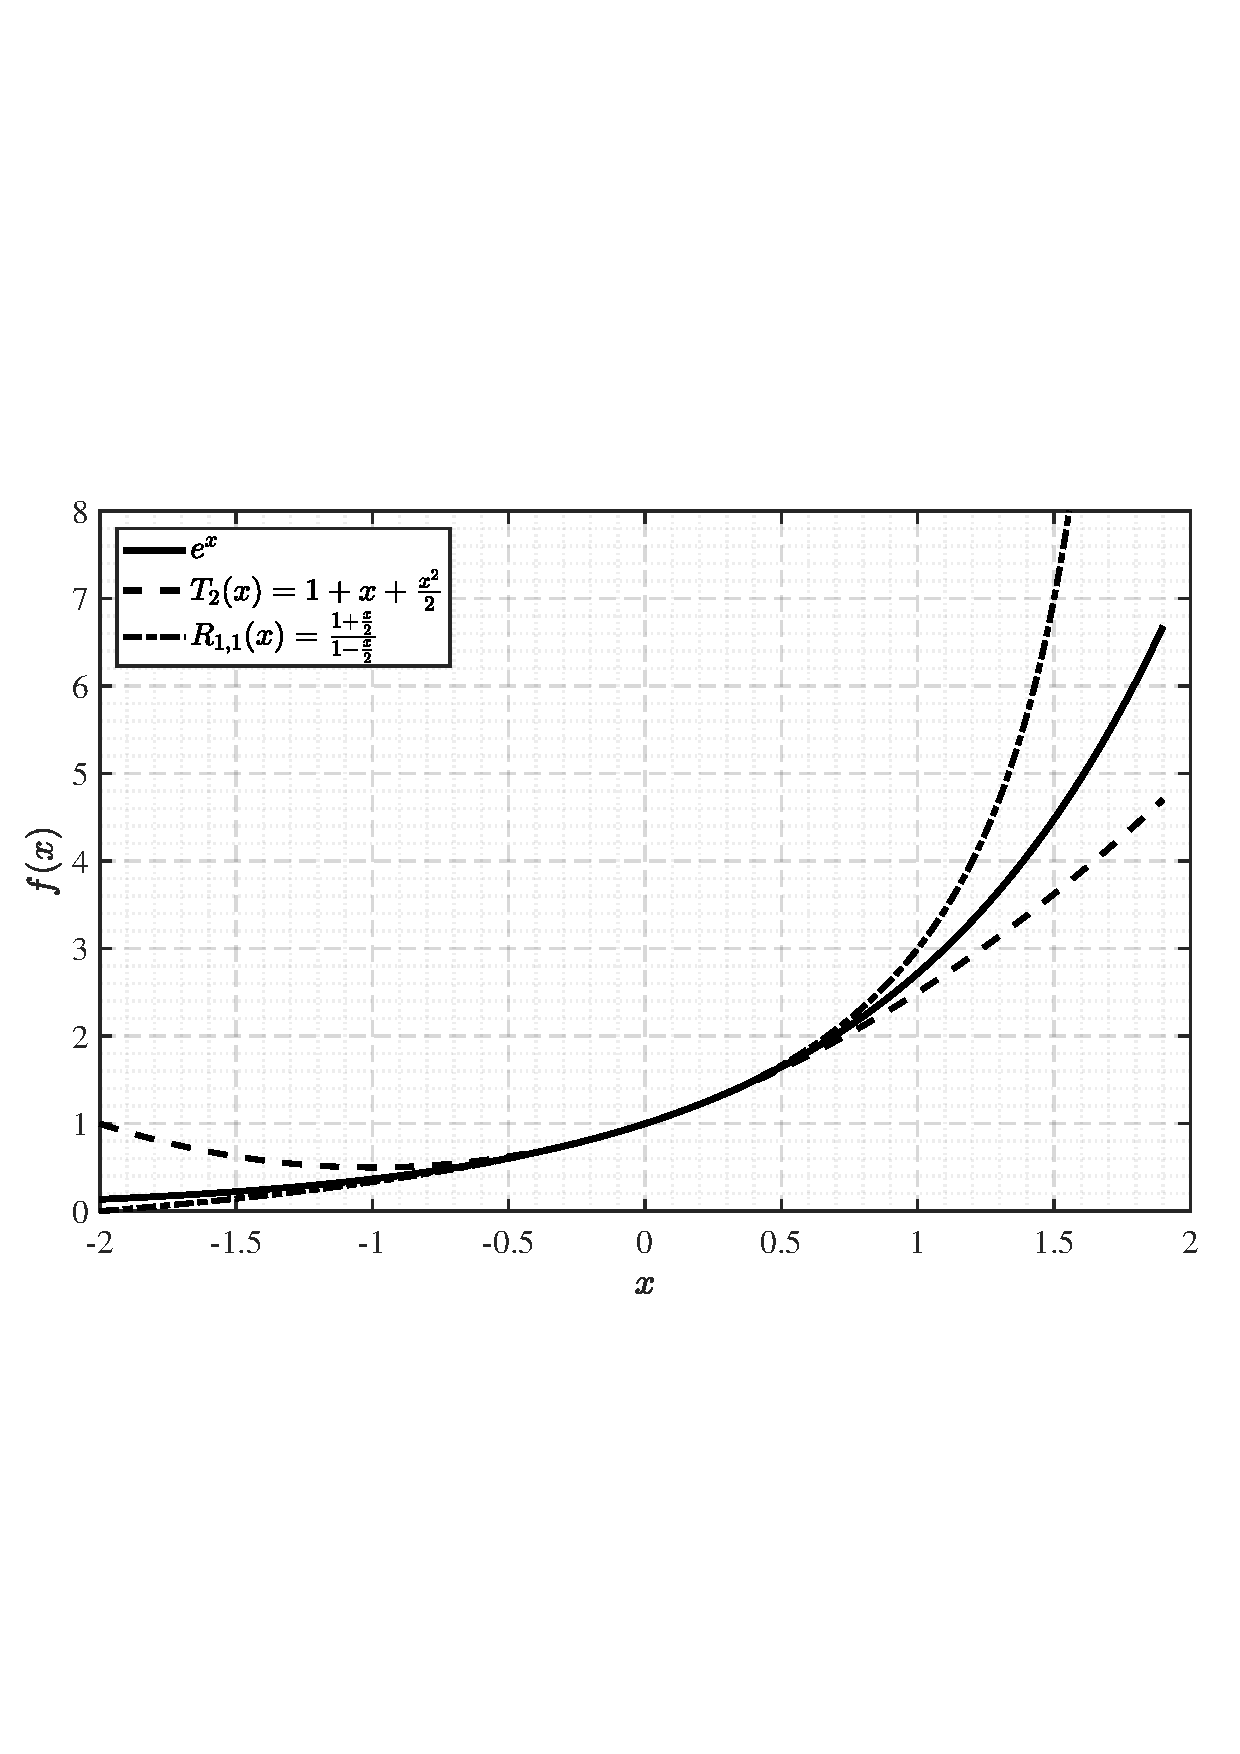
\includegraphics[width=\textwidth]{papers/pade/images/vergleich.pdf}};
\end{tikzpicture}
\caption{TODO
\label{pade:fig:vergleich}}
\end{figure}

In der unmittelbaren Umgebung des Entwicklungspunktes stimmen beide Approximationen nahezu mit der Exponentialfunktion überein. Mit zunehmendem Abstand wird jedoch deutlich, dass die Padé-Approximation den Verlauf der Exponentialfunktion besser beschreibt als das Taylor-Polynom.

Der Grund hierfür liegt in der mathematischen Struktur der Approximation. Während ein Taylor-Polynom ausschliesslich aus Potenzen der Variablen besteht, besitzt die Padé-Approximation zusätzlich ein Nennerpolynom. Dadurch stehen weitere Freiheitsgrade zur Verfügung, welche eine bessere Anpassung an den Funktionsverlauf ermöglichen.

Die Padé-[1/1]-Approximation besitzt allerdings auch Einschränkungen. Da ihr Nenner \(1-\frac{x}{2}\) für \(x=2\) verschwindet, besitzt die Approximation an dieser Stelle eine Polstelle. Die Exponentialfunktion selbst besitzt keine Polstellen. Man spricht deshalb von einer künstlichen Polstelle, welche ausschliesslich durch die Approximation entsteht.

Dieses Beispiel zeigt, dass auch Padé-Approximationen nicht exakt sind. Dennoch liefern sie in vielen Anwendungen eine deutlich bessere Näherung als Taylor-Polynome gleicher Ordnung. Eine weitere Verbesserung kann durch Padé-Approximationen höherer Ordnung erreicht werden.

\subsection{Padé-Approximationen höherer Ordnung}
\label{pade:subsection:hoehere}

Die bisher betrachtete Padé-[1/1]-Approximation verwendet lediglich die ersten drei Koeffizienten der Taylor-Reihe. Soll die Genauigkeit weiter verbessert werden, müssen zusätzliche Informationen der Taylor-Reihe berücksichtigt werden. Dies geschieht durch Padé-Approximationen höherer Ordnung.

Allgemein besitzt eine Padé-Approximation vom Typ \([m/n]\) die Form
\begin{equation}
R_{m,n}(x)
=
\frac
{a_0+a_1x+\cdots+a_mx^m}
{1+b_1x+\cdots+b_nx^n}.
\label{pade:eq:mn}
\end{equation}
Der Zähler besitzt den Grad \(m\), der Nenner den Grad \(n\). Da der konstante Term des Nennerpolynoms auf \(1\) normiert wird, enthält die Approximation insgesamt \(m+n+1\) unbekannte Koeffizienten.

Zur Bestimmung dieser Koeffizienten wird wiederum die Taylor-Reihe der ursprünglichen Funktion verwendet. Allgemein gilt
\begin{equation}
f(x)-R_{m,n}(x)
=
O(x^{m+n+1}).
\label{pade:eq:ordnung2}
\end{equation}
Dies bedeutet, dass die Taylor-Reihe der Funktion und die Reihenentwicklung der Padé-Approximation bis einschliesslich des Terms \(x^{m+n}\) übereinstimmen. Erst ab höheren Potenzen treten Unterschiede auf.

Als Beispiel wird nun die Padé-Approximation vom Typ \([2/2]\) betrachtet. Sie besitzt die Form
\begin{equation}
R_{2,2}(x)
=
\frac
{a_0+a_1x+a_2x^2}
{1+b_1x+b_2x^2}.
\label{pade:eq:pade22_ansatz}
\end{equation}

Im Vergleich zur Padé-[1/1]-Approximation treten nun insgesamt fünf unbekannte Koeffizienten auf. Nach der Entwicklung des Nenners, dem Ausmultiplizieren sowie dem Koeffizientenvergleich erhält man das entsprechende lineare Gleichungssystem. Die vollständige Herleitung erfolgt analog zur Padé-[1/1]-Approximation und wird deshalb an dieser Stelle nicht vollständig ausgeschrieben.

Für die Exponentialfunktion ergeben sich die Koeffizienten
\begin{align}
a_0 &= 1,\\
a_1 &= \frac12,\\
a_2 &= \frac1{12},\\
b_1 &= -\frac12,\\
b_2 &= \frac1{12}.
\end{align}

Damit erhält man die Padé-[2/2]-Approximation
\begin{equation}
R_{2,2}(x)
=
\frac
{1+\frac{x}{2}+\frac{x^2}{12}}
{1-\frac{x}{2}+\frac{x^2}{12}}.
\label{pade:eq:pade22}
\end{equation}

Im Vergleich zur Padé-[1/1]-Approximation werden nun mehr Koeffizienten der Taylor-Reihe exakt reproduziert. Dadurch verbessert sich die Genauigkeit der Approximation über einen grösseren Bereich.

Abbildung~\ref{pade:fig:pade22} zeigt den Vergleich zwischen der Exponentialfunktion sowie den Padé-Approximationen erster und zweiter Ordnung.

%Bild 3, Teil3, (pade22), e^x vs Pade 1-1 u 2-2
\begin{figure}
\centering
\begin{tikzpicture}
\clip (-6.3,-4) rectangle (6.3,4);
\node at (0,0) {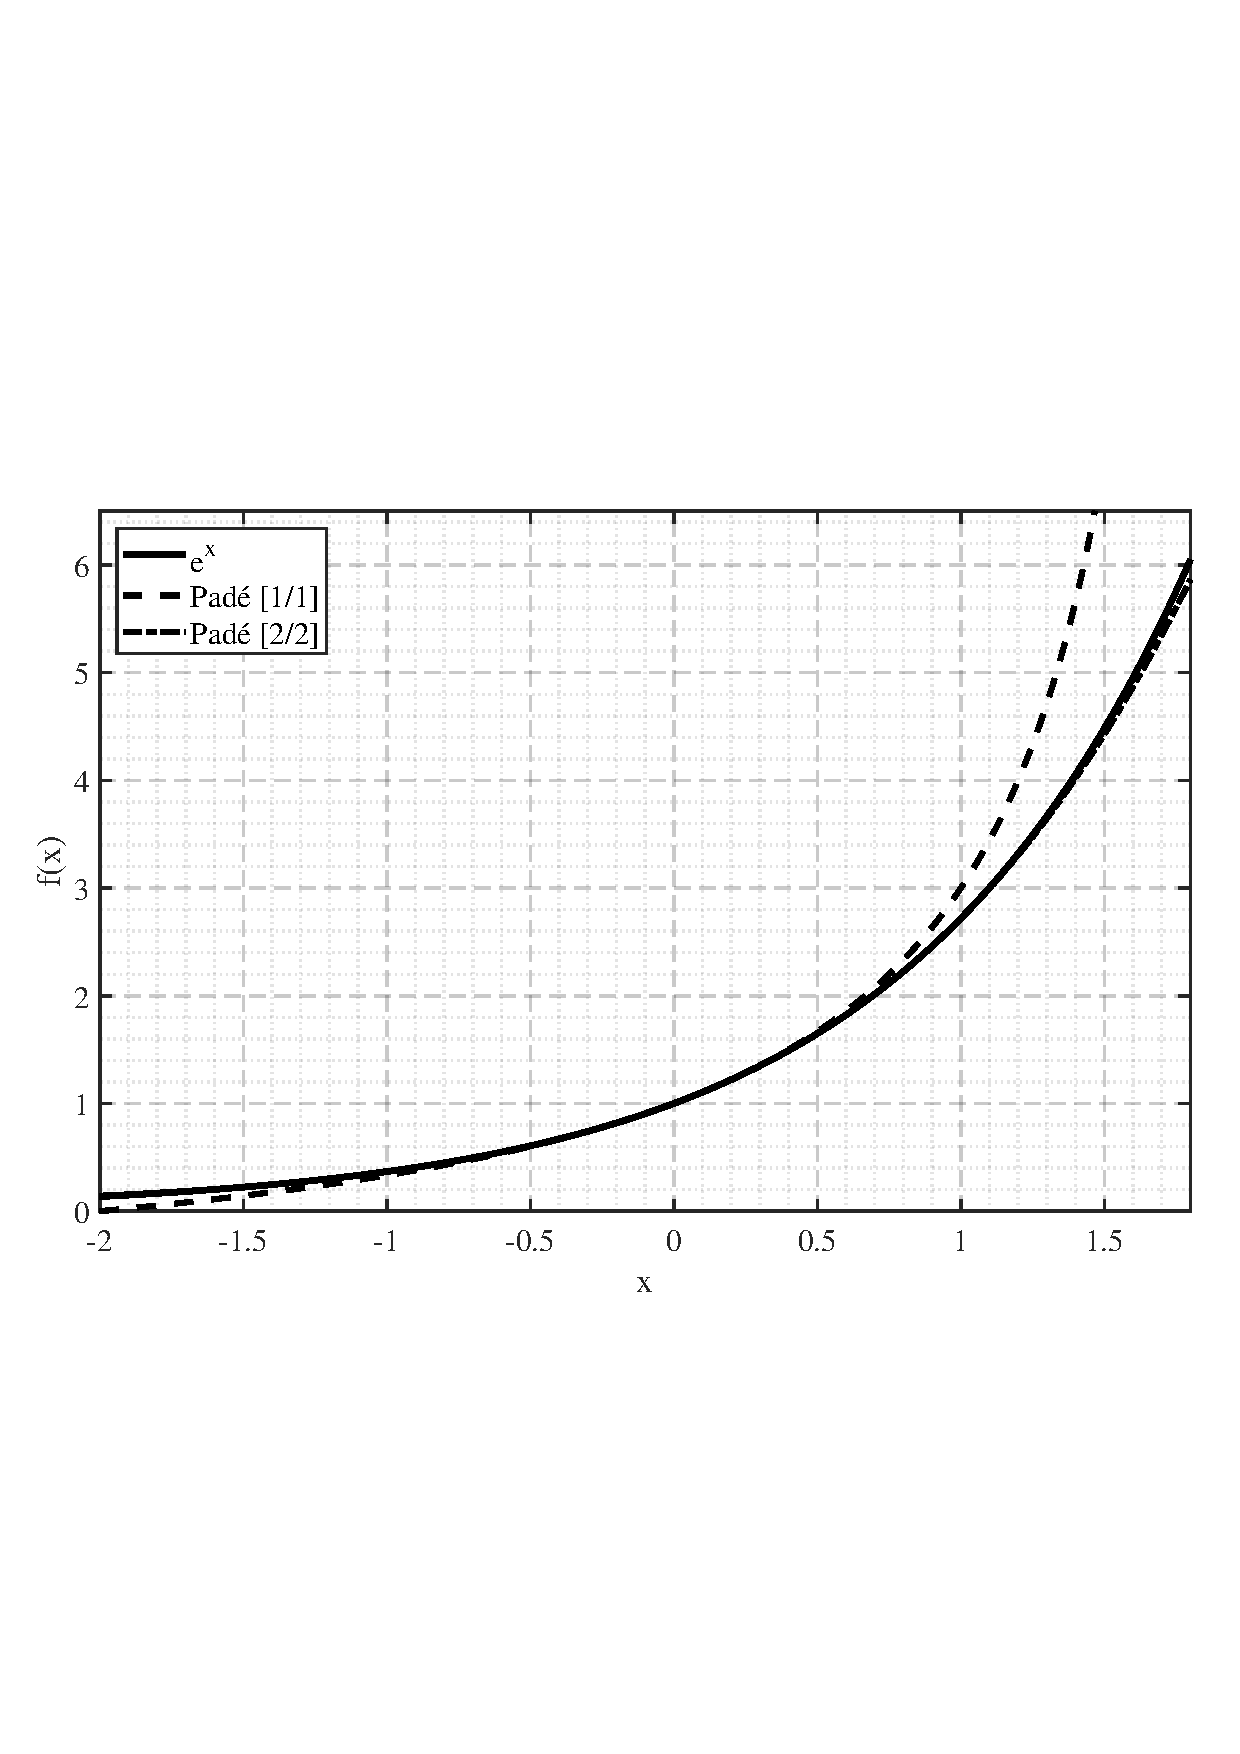
\includegraphics[width=\textwidth]{papers/pade/images/pade22.pdf}};
\end{tikzpicture}
\caption{TODO
\label{pade:fig:pade22}}
\end{figure}

Wie zu erwarten, nähert sich die Padé-[2/2]-Approximation dem exakten Funktionsverlauf über einen deutlich grösseren Bereich an als die Padé-[1/1]-Approximation. Mit steigender Ordnung verbessert sich die Approximation im Allgemeinen weiter, gleichzeitig nimmt jedoch auch der Rechenaufwand zur Bestimmung der Koeffizienten zu.

Im letzten Abschnitt dieses Kapitels werden die wichtigsten Anwendungsgebiete der Padé-Approximation vorgestellt sowie ihre Vor- und Nachteile zusammengefasst.

\subsection{Anwendungen der Padé-Approximation}
\label{pade:subsection:anwendungen}

Nachdem die mathematischen Grundlagen der Padé-Approximation vorgestellt wurden, stellt sich die Frage nach ihrer praktischen Bedeutung. Obwohl das Verfahren ursprünglich im Rahmen der Approximationstheorie entwickelt wurde, findet es heute in zahlreichen wissenschaftlichen und technischen Anwendungen Verwendung. Überall dort, wo Funktionen effizient und gleichzeitig mit hoher Genauigkeit ausgewertet werden müssen, kann die Padé-Approximation ihre Stärken ausspielen.

Eine wichtige Anwendung findet sich in der numerischen Mathematik. Viele elementare Funktionen wie die Exponentialfunktion, der natürliche Logarithmus oder trigonometrische Funktionen werden in numerischen Algorithmen nicht direkt berechnet, sondern durch Approximationen ersetzt. Padé-Approximationen liefern dabei häufig genauere Ergebnisse als Taylor-Polynome gleicher Ordnung und werden deshalb in verschiedenen numerischen Verfahren eingesetzt.

Ein weiteres bedeutendes Anwendungsgebiet ist die Regelungstechnik. Viele technische Systeme besitzen sogenannte Totzeiten. Zwischen einer Änderung der Eingangsgrösse und der Reaktion des Systems vergeht dabei eine bestimmte Zeit. Im Laplace-Bereich wird eine Totzeit durch
\begin{equation}
e^{-sT}
\label{pade:eq:totzeit}
\end{equation}
beschrieben.

Da diese Exponentialfunktion analytische Berechnungen erschwert, wird sie häufig durch eine Padé-Approximation ersetzt. Für eine Padé-[1/1]-Approximation ergibt sich
\begin{equation}
e^{-sT}
\approx
\frac{1-\frac{sT}{2}}
{1+\frac{sT}{2}}.
\label{pade:eq:totzeit_pade}
\end{equation}
Dadurch entsteht eine rationale Übertragungsfunktion, welche sich mit den Methoden der klassischen Regelungstechnik wesentlich einfacher untersuchen lässt.

Abbildung~\ref{pade:fig:totzeit} zeigt beispielhaft den Vergleich zwischen der exakten Sprungantwort einer Totzeit und der entsprechenden Padé-[1/1]-Approximation.

%Bild 4, Teil3, (totzeit), Pade von Totzeit
\begin{figure}
\centering
\begin{tikzpicture}
\clip (-6.3,-4.9) rectangle (6.3,4.3);
\node at (0,0) {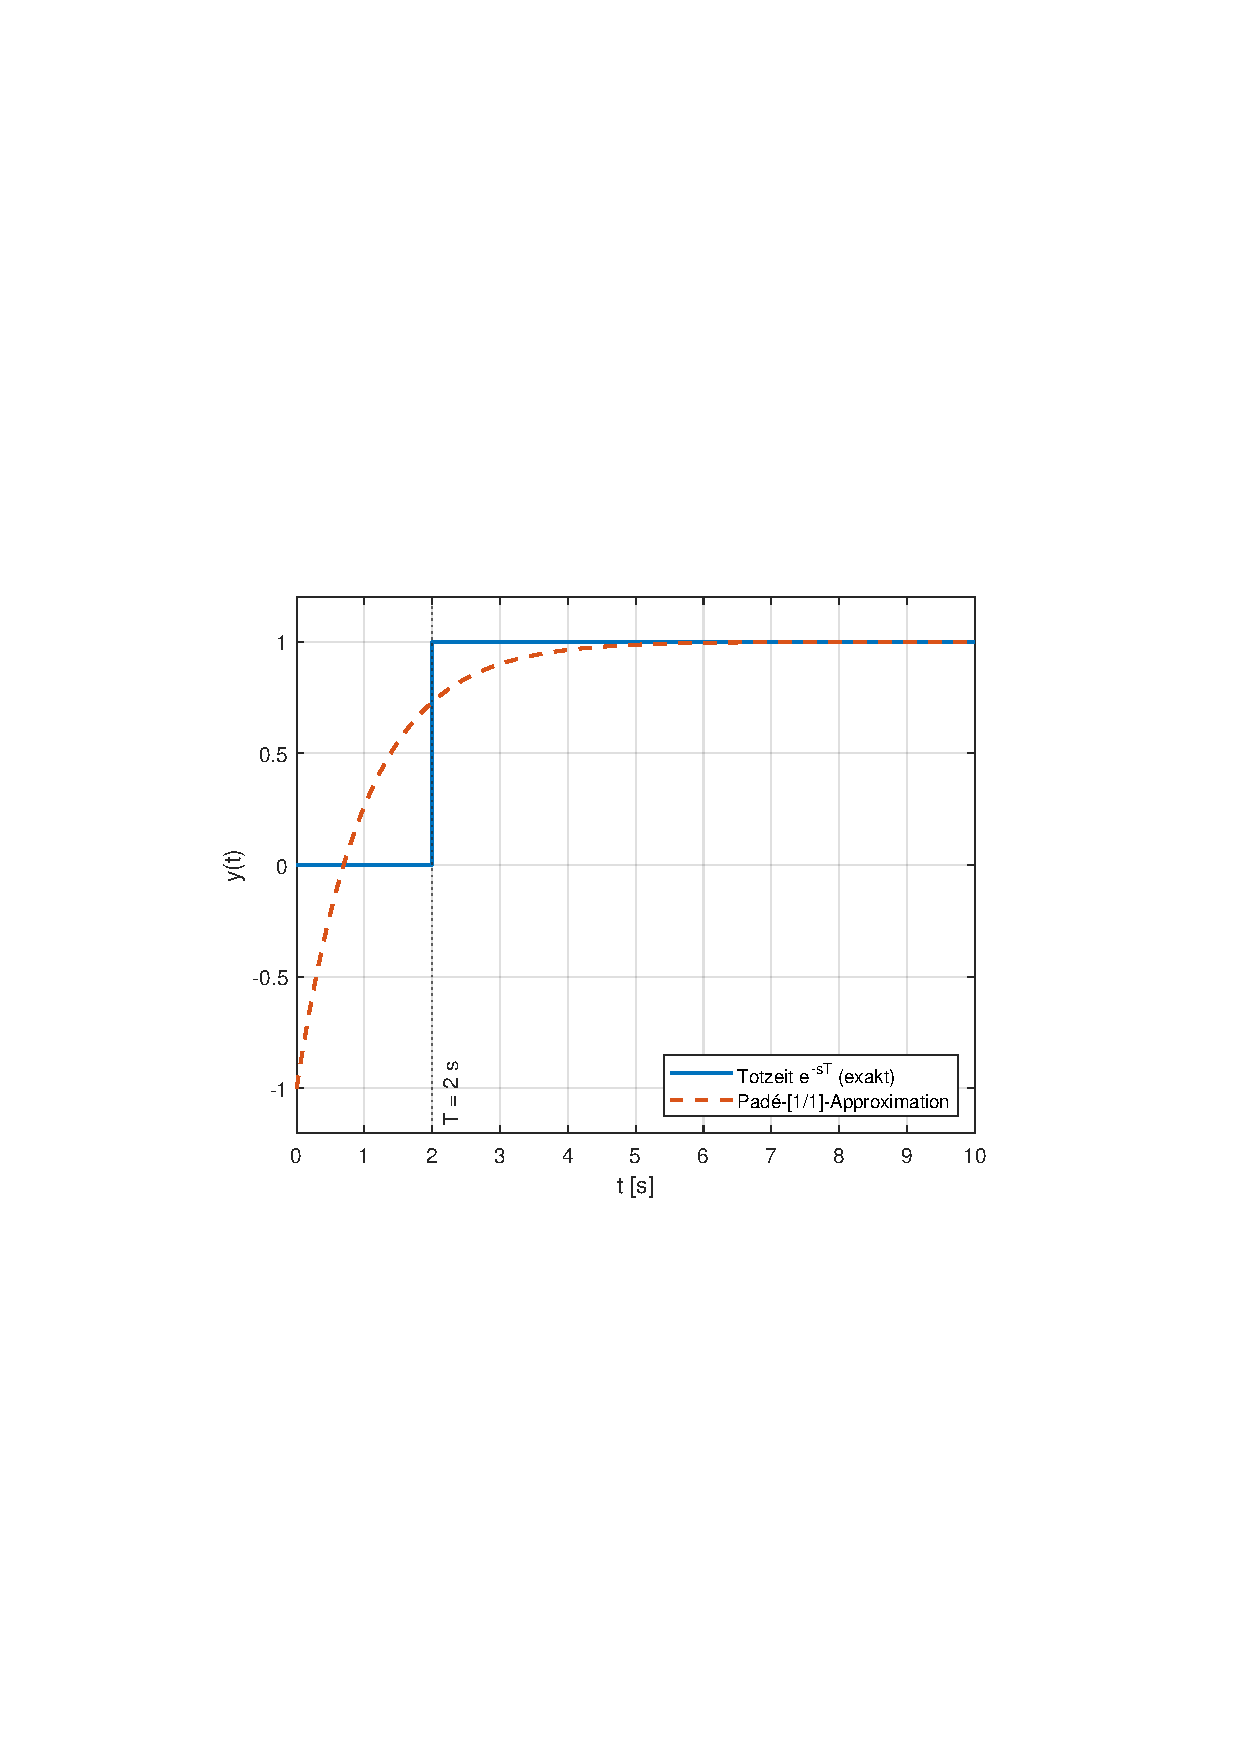
\includegraphics[width=1.5\textwidth]{papers/pade/images/totzeit.pdf}};
\end{tikzpicture}
\caption{TODO
\label{pade:fig:totzeit}}
\end{figure}

Auch bei der numerischen Lösung gewöhnlicher und partieller Differentialgleichungen werden Padé-Approximationen eingesetzt. Häufig wird zunächst eine Taylor-Reihe der Lösung bestimmt und anschliessend in eine Padé-Approximation umgewandelt. Dadurch kann die Lösung oftmals über einen grösseren Bereich mit höherer Genauigkeit beschrieben werden.

Darüber hinaus finden Padé-Approximationen zahlreiche Anwendungen in der theoretischen Physik. Insbesondere in der Quantenmechanik, der statistischen Physik und der Strömungsmechanik treten Reihenentwicklungen auf, deren Konvergenzbereich begrenzt ist. Durch die Umwandlung dieser Reihen in rationale Funktionen lassen sich häufig genauere numerische Ergebnisse erzielen.

Ein weiterer Vorteil der Padé-Approximation zeigt sich darin, dass sie nicht auf reelle Argumente beschränkt ist. Da sie für Funktionen mit konvergenter Potenzreihe konstruiert werden kann, besitzen insbesondere holomorphe Funktionen eine Padé-Approximation. Damit liefert die Padé-Approximation nicht nur für reelle, sondern auch für komplexe Werte eine Näherung.

Ein anschauliches Beispiel liefert erneut die Exponentialfunktion. Für ein komplexes Argument \(z=ix\) gilt \(e^{ix}=\cos(x)+i\sin(x)\). Eine Padé-Approximation der Exponentialfunktion kann deshalb auch zur Approximation von Sinus und Kosinus verwendet werden. Abbildung~\ref{pade:fig:komplex} zeigt den Vergleich zwischen den exakten Funktionen und den aus der Padé-[1/1]-Approximation gewonnenen Real- und Imaginärteilen.

%Bild 5, Teil3, (komplex), Pade Komplex
\begin{figure}
\centering
\begin{tikzpicture}
\clip (-6.3,-4.9) rectangle (6.3,4.3);
\node at (0,0) {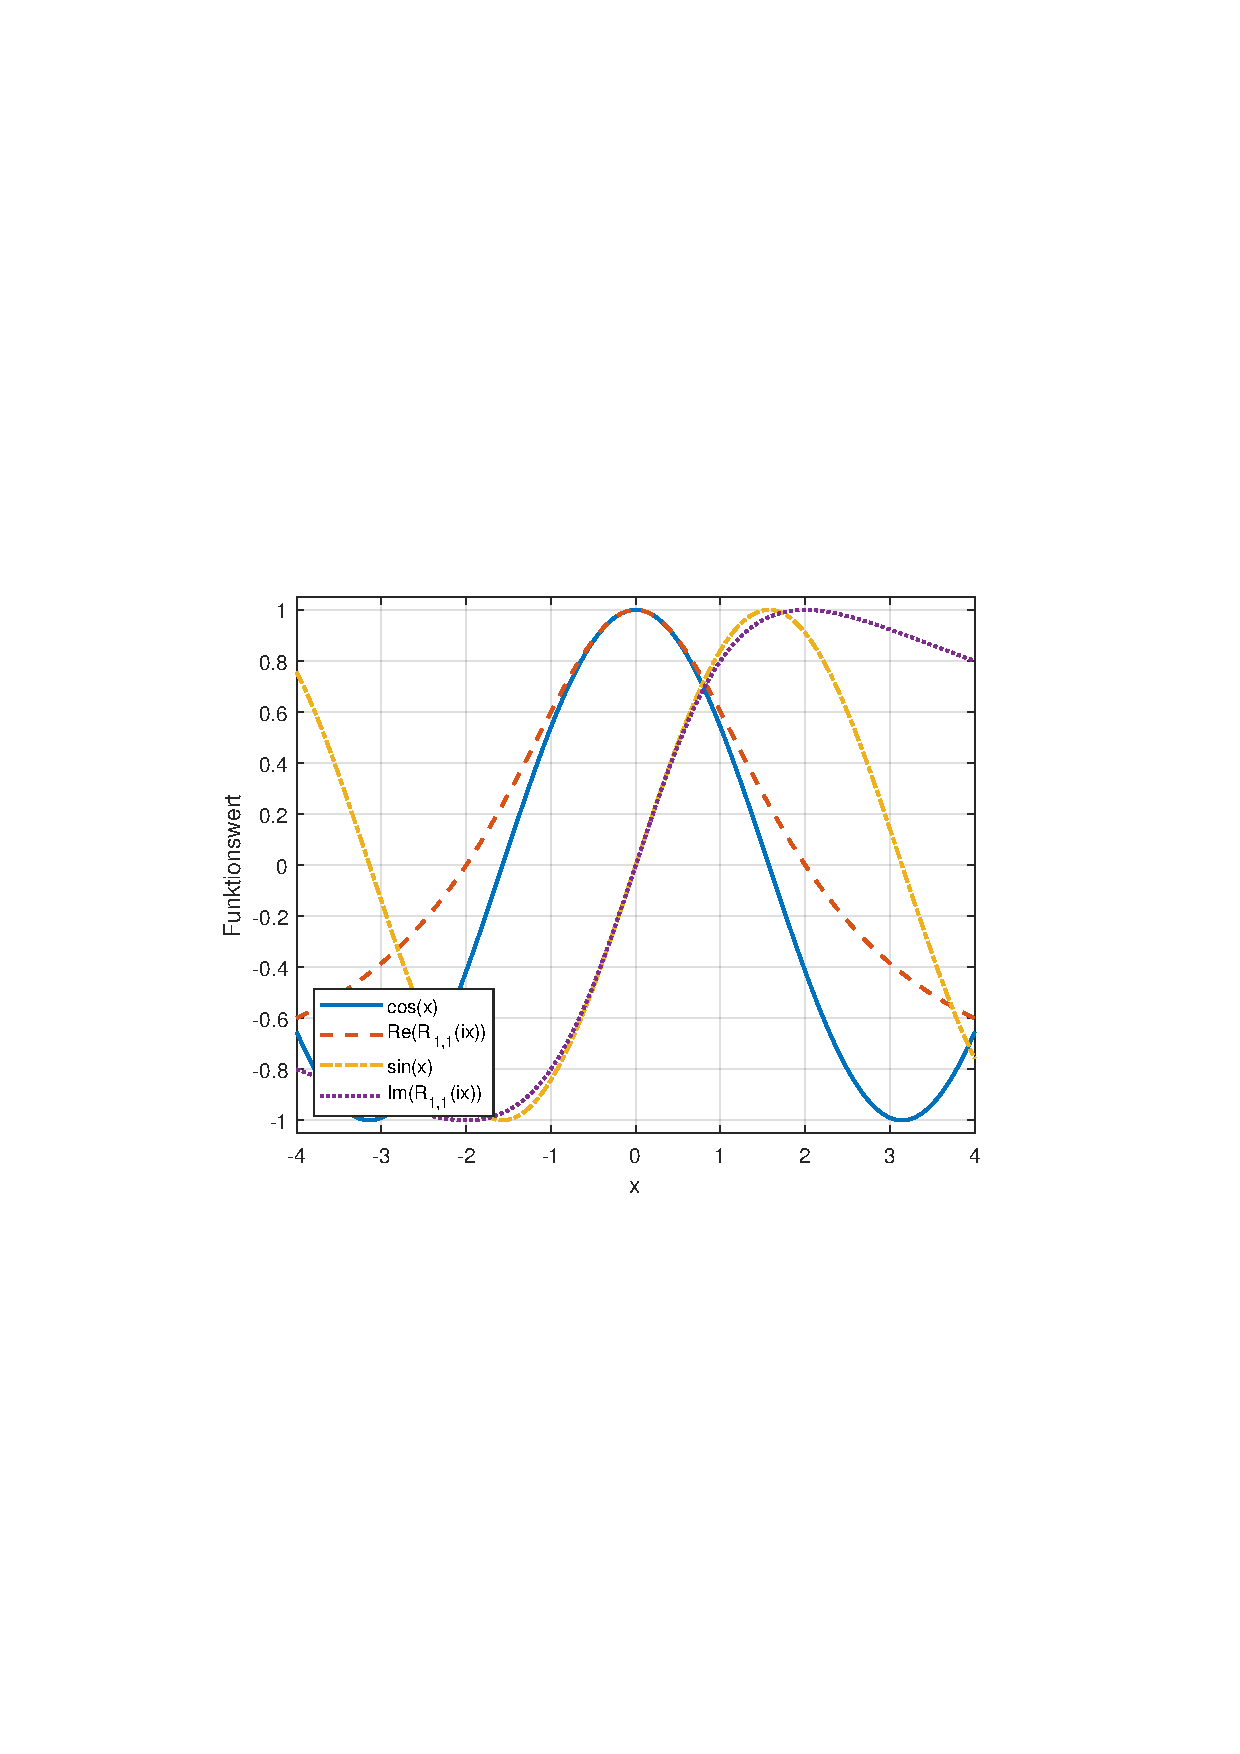
\includegraphics[width=1.5\textwidth]{papers/pade/images/komplex.pdf}};
\end{tikzpicture}
\caption{TODO
\label{pade:fig:komplex}}
\end{figure}

Ein weiterer Vorteil besteht darin, dass die Padé-Approximation die aus der Taylor-Reihe bekannte Ableitungsinformation erhält. Da die Reihenentwicklung der Padé-Approximation bis zur geforderten Ordnung mit jener der ursprünglichen Funktion übereinstimmt, stimmen auch die entsprechenden Ableitungen am Entwicklungspunkt überein. Die Ableitung einer Padé-Approximation liefert somit wiederum eine Approximation der Ableitung der ursprünglichen Funktion.

Bei herkömmlichen Interpolationsverfahren ist diese Eigenschaft nicht automatisch gegeben. Soll eine Funktion und gleichzeitig ihre Ableitung an bestimmten Stellen approximiert werden, muss beispielsweise eine spezielle Methode wie die Hermite-Interpolation verwendet werden.

\subsection{Vor- und Nachteile}
\label{pade:subsection:vorteile}

Wie jedes Approximationsverfahren besitzt auch die Padé-Approximation sowohl Vorteile als auch Einschränkungen.

Ein wesentlicher Vorteil besteht darin, dass ausschliesslich die Koeffizienten der Taylor-Reihe benötigt werden. Zusätzliche Informationen über die Funktion sind nicht erforderlich. Durch die Darstellung als rationale Funktion kann der Verlauf vieler Funktionen genauer beschrieben werden als mit einem Taylor-Polynom gleicher Ordnung.

Insbesondere ausserhalb der unmittelbaren Umgebung des Entwicklungspunktes liefern Padé-Approximationen häufig deutlich kleinere Approximationsfehler. Darüber hinaus können rationale Funktionen Eigenschaften beschreiben, welche mit Polynomen grundsätzlich nicht dargestellt werden können, beispielsweise asymptotisches Verhalten.

Demgegenüber stehen jedoch auch einige Nachteile. Je höher die Ordnung der Padé-Approximation gewählt wird, desto grösser wird das zu lösende lineare Gleichungssystem und damit auch der Rechenaufwand. Zudem können künstliche Polstellen entstehen, welche in der ursprünglichen Funktion nicht vorhanden sind.

Die wichtigsten Eigenschaften beider Verfahren sind in Tabelle~\ref{pade:tab:vor_nachteile} zusammengefasst.

\begin{table}[ht]
\centering
\caption{Vergleich zwischen Taylor- und Padé-Approximation.}
\label{pade:tab:vor_nachteile}
\begin{tabular}{lll}
\hline
Eigenschaft & Taylor & Padé\\
\hline
Grundlage & Taylor-Reihe & Taylor-Reihe\\
Darstellung & Polynom & rationale Funktion\\
Genauigkeit & lokal sehr gut & häufig auf grösserem Bereich\\
Polstellen & keine & künstliche Polstellen möglich\\
Rechenaufwand & gering & höher\\
Anwendungen & lokale Approximation & Numerik, Regelungstechnik, Physik\\
\hline
\end{tabular}
\end{table}
